% Hinh FLOW: giao thuc hai arm + phep giao + phan dung lai.
% Bo style nha: paper-lab/transaction-figure-kit/flow/txstyle.tex
%
% ⛔ BA LOI CUA BAN TRUOC, chi thay khi KET XUAT PNG VA NHIN, khong cong nao bat duoc:
%   1. hop chu thich dai hon `minimum width` nen no NO RA HAI BEN va tran khoi vung MEASURE.
%      Sua bang `text width` de chu XUONG DONG thay vi day khung rong ra.
%   2. mui ten tu Arm B chay THANG QUA hop "does position..." va gach ngang chu trong do.
%      Sua bang cach dinh tuyen qua mot cot doc rieng ben phai vung MEASURE.
%   3. hop cuoi cua Arm B khong co mui ten noi.
% ⚠ Bo cuc phai vua kho chu LNCS (4,80 in). Xem check_figure_scale.
\documentclass[tikz,border=2pt]{standalone}
\usepackage[T1]{fontenc}
\usepackage{tikz}
% =====================================================================
%  Transaction-grade TikZ style kit (flow / architecture figures)
%  Triết lý: nền xám trắng, 1 màu nhấn cho khối Đề xuất, nét mảnh đều,
%  góc vuông/bo rất nhẹ, mũi tên một trọng số, không bóng/gradient.
%  % =====================================================================
%  Transaction-grade TikZ style kit (flow / architecture figures)
%  Triết lý: nền xám trắng, 1 màu nhấn cho khối Đề xuất, nét mảnh đều,
%  góc vuông/bo rất nhẹ, mũi tên một trọng số, không bóng/gradient.
%  % =====================================================================
%  Transaction-grade TikZ style kit (flow / architecture figures)
%  Triết lý: nền xám trắng, 1 màu nhấn cho khối Đề xuất, nét mảnh đều,
%  góc vuông/bo rất nhẹ, mũi tên một trọng số, không bóng/gradient.
%  \input{txstyle.tex} sau \usepackage{tikz}.
% =====================================================================
\usetikzlibrary{arrows.meta, positioning, fit, backgrounds, calc}

% ---- ONE accent color per paper (đổi mã HEX này theo từng bài) ----
\definecolor{accent}{HTML}{2C6E9B}   % muted steel blue
\definecolor{inkgray}{HTML}{3A3F47}

\tikzset{
  >={Latex[length=2mm, width=1.6mm]},
  font=\footnotesize,
  % --- khối thường: xám rất nhạt, góc vuông, nét 0.5pt ---
  blk/.style={draw=inkgray, line width=0.5pt, fill=black!3,
              minimum width=22mm, minimum height=10mm, align=center,
              inner sep=3pt, rounded corners=0.6pt},
  % --- khối ĐỀ XUẤT: nhấn accent nhẹ, nét đậm hơn chút ---
  prop/.style={blk, draw=accent, fill=accent!7, line width=0.8pt},
  % --- node nhỏ (vệ tinh / cell) ---
  sml/.style={draw=inkgray, line width=0.5pt, fill=black!3,
              minimum width=16mm, minimum height=8mm, align=center,
              inner sep=2pt, font=\scriptsize, rounded corners=0.6pt},
  % --- luồng dữ liệu (liền) và hồi tiếp/điều khiển (đứt) ---
  flow/.style={->, draw=inkgray, line width=0.55pt},
  fb/.style={->, draw=inkgray!75, line width=0.55pt, dashed, dash pattern=on 3pt off 2pt},
  % --- nhãn cạnh mũi tên: nhỏ, nghiêng, xám ---
  alab/.style={font=\scriptsize\itshape, text=inkgray!75, inner sep=1.5pt},
  % --- vùng nhóm: khung đứt mảnh + nhãn in hoa nhỏ ---
  zone/.style={draw=inkgray!45, line width=0.4pt, dashed,
               dash pattern=on 2pt off 2pt, inner sep=4mm, rounded corners=1pt},
  zlab/.style={font=\scriptsize\bfseries, text=inkgray!70},
}
 sau \usepackage{tikz}.
% =====================================================================
\usetikzlibrary{arrows.meta, positioning, fit, backgrounds, calc}

% ---- ONE accent color per paper (đổi mã HEX này theo từng bài) ----
\definecolor{accent}{HTML}{2C6E9B}   % muted steel blue
\definecolor{inkgray}{HTML}{3A3F47}

\tikzset{
  >={Latex[length=2mm, width=1.6mm]},
  font=\footnotesize,
  % --- khối thường: xám rất nhạt, góc vuông, nét 0.5pt ---
  blk/.style={draw=inkgray, line width=0.5pt, fill=black!3,
              minimum width=22mm, minimum height=10mm, align=center,
              inner sep=3pt, rounded corners=0.6pt},
  % --- khối ĐỀ XUẤT: nhấn accent nhẹ, nét đậm hơn chút ---
  prop/.style={blk, draw=accent, fill=accent!7, line width=0.8pt},
  % --- node nhỏ (vệ tinh / cell) ---
  sml/.style={draw=inkgray, line width=0.5pt, fill=black!3,
              minimum width=16mm, minimum height=8mm, align=center,
              inner sep=2pt, font=\scriptsize, rounded corners=0.6pt},
  % --- luồng dữ liệu (liền) và hồi tiếp/điều khiển (đứt) ---
  flow/.style={->, draw=inkgray, line width=0.55pt},
  fb/.style={->, draw=inkgray!75, line width=0.55pt, dashed, dash pattern=on 3pt off 2pt},
  % --- nhãn cạnh mũi tên: nhỏ, nghiêng, xám ---
  alab/.style={font=\scriptsize\itshape, text=inkgray!75, inner sep=1.5pt},
  % --- vùng nhóm: khung đứt mảnh + nhãn in hoa nhỏ ---
  zone/.style={draw=inkgray!45, line width=0.4pt, dashed,
               dash pattern=on 2pt off 2pt, inner sep=4mm, rounded corners=1pt},
  zlab/.style={font=\scriptsize\bfseries, text=inkgray!70},
}
 sau \usepackage{tikz}.
% =====================================================================
\usetikzlibrary{arrows.meta, positioning, fit, backgrounds, calc}

% ---- ONE accent color per paper (đổi mã HEX này theo từng bài) ----
\definecolor{accent}{HTML}{2C6E9B}   % muted steel blue
\definecolor{inkgray}{HTML}{3A3F47}

\tikzset{
  >={Latex[length=2mm, width=1.6mm]},
  font=\footnotesize,
  % --- khối thường: xám rất nhạt, góc vuông, nét 0.5pt ---
  blk/.style={draw=inkgray, line width=0.5pt, fill=black!3,
              minimum width=22mm, minimum height=10mm, align=center,
              inner sep=3pt, rounded corners=0.6pt},
  % --- khối ĐỀ XUẤT: nhấn accent nhẹ, nét đậm hơn chút ---
  prop/.style={blk, draw=accent, fill=accent!7, line width=0.8pt},
  % --- node nhỏ (vệ tinh / cell) ---
  sml/.style={draw=inkgray, line width=0.5pt, fill=black!3,
              minimum width=16mm, minimum height=8mm, align=center,
              inner sep=2pt, font=\scriptsize, rounded corners=0.6pt},
  % --- luồng dữ liệu (liền) và hồi tiếp/điều khiển (đứt) ---
  flow/.style={->, draw=inkgray, line width=0.55pt},
  fb/.style={->, draw=inkgray!75, line width=0.55pt, dashed, dash pattern=on 3pt off 2pt},
  % --- nhãn cạnh mũi tên: nhỏ, nghiêng, xám ---
  alab/.style={font=\scriptsize\itshape, text=inkgray!75, inner sep=1.5pt},
  % --- vùng nhóm: khung đứt mảnh + nhãn in hoa nhỏ ---
  zone/.style={draw=inkgray!45, line width=0.4pt, dashed,
               dash pattern=on 2pt off 2pt, inner sep=4mm, rounded corners=1pt},
  zlab/.style={font=\scriptsize\bfseries, text=inkgray!70},
}

\definecolor{accent}{HTML}{2C6E9B}
\begin{document}
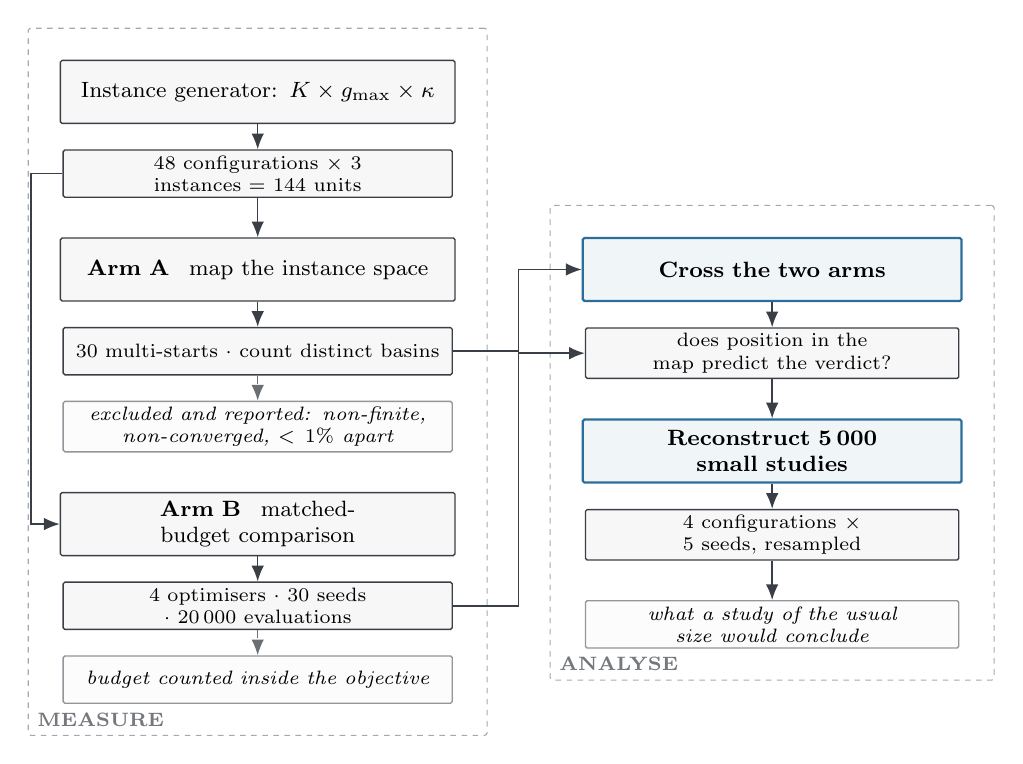
\begin{tikzpicture}[node distance=3.2mm,
   blk/.append style={text width=48mm, align=center, minimum height=8mm},
   sml/.append style={text width=48mm, align=center, minimum height=6mm, font=\scriptsize},
   note/.style={sml, fill=black!1, draw=inkgray!55, font=\scriptsize\itshape},
   prop/.append style={text width=46mm, align=center, minimum height=8mm}]

% ================= cot trai: DO =================
\node[blk] (gen) {Instance generator: $K \times g_{\max} \times \kappa$};
\node[sml, below=of gen] (unit) {48 configurations $\times$ 3 instances $=$ 144 units};
\node[blk, below=5mm of unit] (armA) {\textbf{Arm A} \, map the instance space};
\node[sml, below=of armA] (armAs) {30 multi-starts $\cdot$ count distinct basins};
\node[note, below=of armAs] (excl)
  {excluded and reported: non-finite, non-converged, $<\!1\%$ apart};
\node[blk, below=5mm of excl] (armB) {\textbf{Arm B} \, matched-budget comparison};
\node[sml, below=of armB] (armBs) {4 optimisers $\cdot$ 30 seeds $\cdot$ 20\,000 evaluations};
\node[note, below=of armBs] (cnt) {budget counted inside the objective};

\draw[flow] (gen) -- (unit);
\draw[flow] (unit) -- (armA);
\draw[flow] (armA) -- (armAs);
\draw[fb]   (armAs) -- (excl);
\draw[flow] (armB) -- (armBs);
\draw[fb]   (armBs) -- (cnt);
\draw[flow] (unit.west) -- ++(-4mm,0) |- (armB.west);

% ================= cot phai: PHAN TICH =================
\node[prop, right=16mm of armA] (cross) {\textbf{Cross the two arms}};
\node[sml, below=of cross, text width=46mm] (crosss)
  {does position in the map predict the verdict?};
\node[prop, below=5mm of crosss] (resamp) {\textbf{Reconstruct 5\,000 small studies}};
\node[sml, below=of resamp, text width=46mm] (resamps)
  {4 configurations $\times$ 5 seeds, resampled};
\node[note, below=5mm of resamps, text width=46mm] (out)
  {what a study of the usual size would conclude};

\draw[flow] (cross) -- (crosss);
\draw[flow] (crosss) -- (resamp);
\draw[flow] (resamp) -- (resamps);
\draw[flow] (resamps) -- (out);

% ⛔ Dinh tuyen qua MOT COT DOC RIENG o x = xr, nam giua hai vung, nen khong mui ten nao
%    cat qua hop nao. Ban truoc di thang tu armBs sang crosss va gach ngang chu trong do.
\coordinate (xr) at ($(armA.east)!0.5!(cross.west)$);
\draw[flow] (armAs.east) -- (armAs.east -| xr) |- (cross.west);
\draw[flow] (armBs.east) -- (armBs.east -| xr) |- (crosss.west);

% ================= vung nhom =================
\begin{scope}[on background layer]
  \node[zone, fit=(gen)(armA)(armAs)(excl)(armB)(armBs)(cnt),
        label={[zlab, anchor=south west]south west:MEASURE}] {};
  \node[zone, fit=(cross)(crosss)(resamp)(resamps)(out),
        label={[zlab, anchor=south west]south west:ANALYSE}] {};
\end{scope}
\end{tikzpicture}
\end{document}
